\documentclass[a4paper, 12pt]{article}
\setlength{\textheight}{24.0cm}
\setlength{\textwidth}{16cm}
\setlength{\parindent}{0.0cm}
\setlength{\topmargin}{-1.0cm}
\setlength{\oddsidemargin}{0.0cm}
\renewcommand{\baselinestretch}{1.4}
    
\usepackage{graphicx}
\usepackage{amsmath}
\usepackage{diffcoeff}
\usepackage{amssymb}
\usepackage{subcaption} 
\usepackage{amsthm}
\usepackage{enumitem}


% Dash int definitions
\def\Xint#1{\mathchoice
{\XXint\displaystyle\textstyle{#1}}%
{\XXint\textstyle\scriptstyle{#1}}%
{\XXint\scriptstyle\scriptscriptstyle{#1}}%
{\XXint\scriptscriptstyle\scriptscriptstyle{#1}}%
\!\int}
\def\XXint#1#2#3{{\setbox0=\hbox{$#1{#2#3}{\int}$ }
\vcenter{\hbox{$#2#3$ }}\kern-.6\wd0}}
\def\ddashint{\Xint=}
\def\dashint{\Xint-}

\numberwithin{equation}{section}
    
\begin{document}
\thispagestyle{empty}
\Large
\vspace*{2cm}
\begin{center}
    \textbf{UNIVERSITY OF STRATHCLYDE}
\end{center}

\vspace*{1cm}
\begin{center}
    \textbf{DEPARTMENT OF\\ MATHEMATICS AND STATISTICS}
\end{center}

\vspace*{1cm}
\begin{center}
    \textbf{THE N-DIMENSIONAL WAVE EQUATION AND THE METHOD OF DESCENT}
\end{center}

\vspace*{1cm}
\begin{center}
    \textbf{by}
\end{center}

\vspace*{1cm}
\begin{center}
    \textbf{IOANA-TEODORA VADUVA}\\
    \textbf{201444379}
\end{center}

\vspace*{3cm}
\begin{center}
    \textbf{BSc Hons Mathematics}
    \textbf{2017/18}
\end{center}

\newpage
\Large

\vspace*{1cm}
\begin{center}
    \textbf{Statement of work in project}
\end{center}

\vspace*{1cm}
\begin{center}
    \parbox{14cm}{
        The work contained in this project is that of the author and where
        material from other sources has been incorporated full acknowledgement
        is made.}
    \end{center}
    
    \begin{center}
        \begin{tabbing}
            xxxxx\=xxxxxxxxxxxxxxx\= \kill
            \\
            \\
            \\
            \>Signed\>.........................................................\\
            \\
            \>Print Name\>.........................................................\\
            \\
            \>Date\>.........................................................\\
        \end{tabbing}
    \end{center}
    
    \vspace*{5cm}
    Supervised by Dr Marcus Waurick
    \newpage
    \normalsize
    \tableofcontents
    \newpage

\section{Introduction}
This project presents the wave equation and its solution in one, two, three and
higher dimensions. The wave equation is a \emph{partial differential equation} (PDE),
an identity that relates independent variables ($x, y...$), a dependent variable
$u$ (a function of the independent variables) and the partial derivatives of
$u$. The wave equation is a PDE of the second order, given by the highest
appearing derivative, see \cite[Ch. 1, \S A]{Fol}. \\

A guitar and a violin make different sounds, despite both being played by
plucking the string. The wave equation allows an insight into how this happens
through an accurate model of the vibrating string. Musical instruments are not,
however, the  only application of the wave equation, which can model accurately
electromagnetic waves, waves in fluids, waves caused by volcanoes and
earthquakes and even has a role in quantum mechanics. Historically, it is of
importance and many representative 18th century mathematicians, D'Alembert,
Euler, Lagrange and Bernoulli, to name a few, had contributions to the
development, modelling and solving of the wave equation, see \cite{Coc}. \\

In this project, we focus our attention on the general wave equation which works
in any number of dimensions. We begin by deriving it from physical principles,
and then focus most of our attention on solving the problem in one, three and
two dimensions, then generalising our result to higher dimensions. We then finish by
proving a uniqueness theorem for our solution.

\section{Derivation of the Wave Equation}
In this section, we will derive the wave equation in one dimension, showing a
pattern that we can extend to higher dimensions. Note that the images in
this section have been created using Adobe Photoshop, but their original
version can be found in \cite[Ch. 12.2]{Kr}.

\subsection{One Dimension}
The wave equation arises from the movement of a string in a musical instrument,
such as a guitar or a violin, see \cite[Ch. 10, App. B]{BoyDiP}. This string is
perfectly elastic, and it is stretched between two supports, at $x=0$ and $x=L$.
The elastic string is of length $L$, as illustrated in Figure \ref{fig:1a}. At
time $t=0$, the string is set into motion and left undisturbed to vibrate in the
vertical plane. For this derivation of the wave equation, we simplify things by
neglecting damping effects such as air resistance and obtain the formula using
the Newtonian mechanics of forces on a small part of the string, of length
$\Delta x$, $\Delta x \in (x, x+\Delta x$, see \cite[Ch. 12.2]{Kr}. Let $u(x,t)$ be the
vertical displacement of point $x$ at the time $t$, $T(x,t)$ - the tension in
the string that acts only in the direction tangent to the string, and $\rho$ the
mass per unit length of the string. 
\begin{figure}[h] 
    \begin{subfigure}[t]{0.5\textwidth} 
        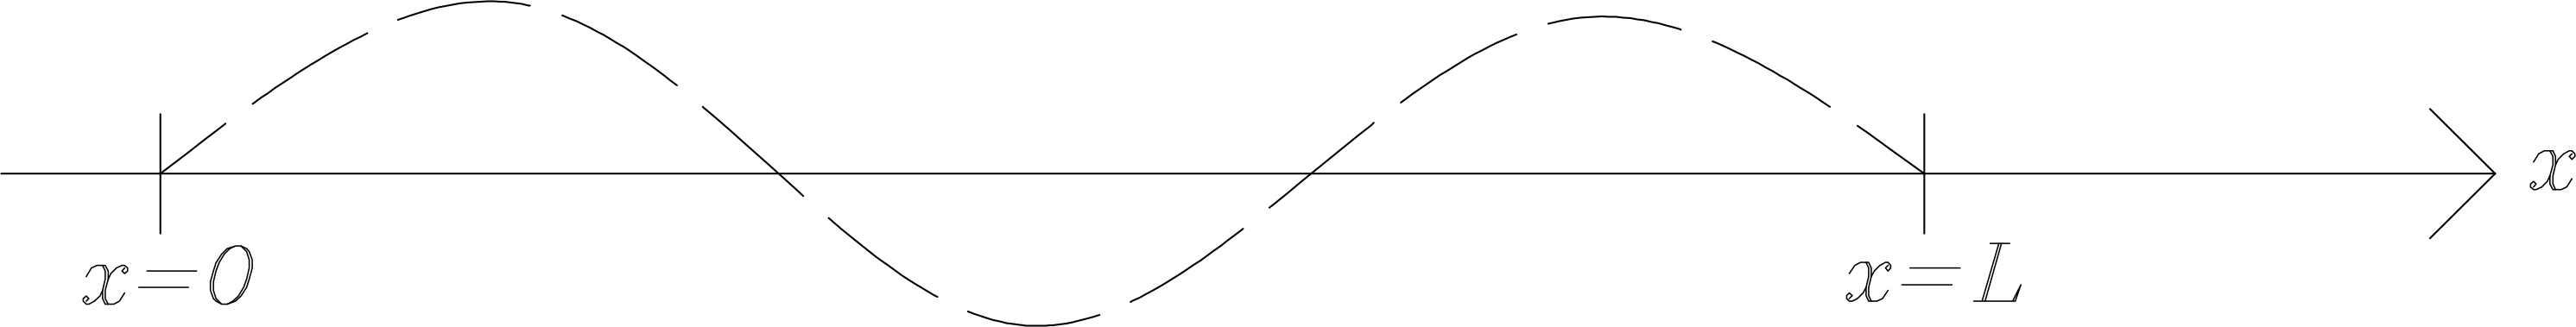
\includegraphics[width=0.9\linewidth]{images/grafic-1.pdf} 
        \caption{String of length L}
        \label{fig:1a}
    \end{subfigure} 
    \begin{subfigure}[t]{0.5\textwidth}
        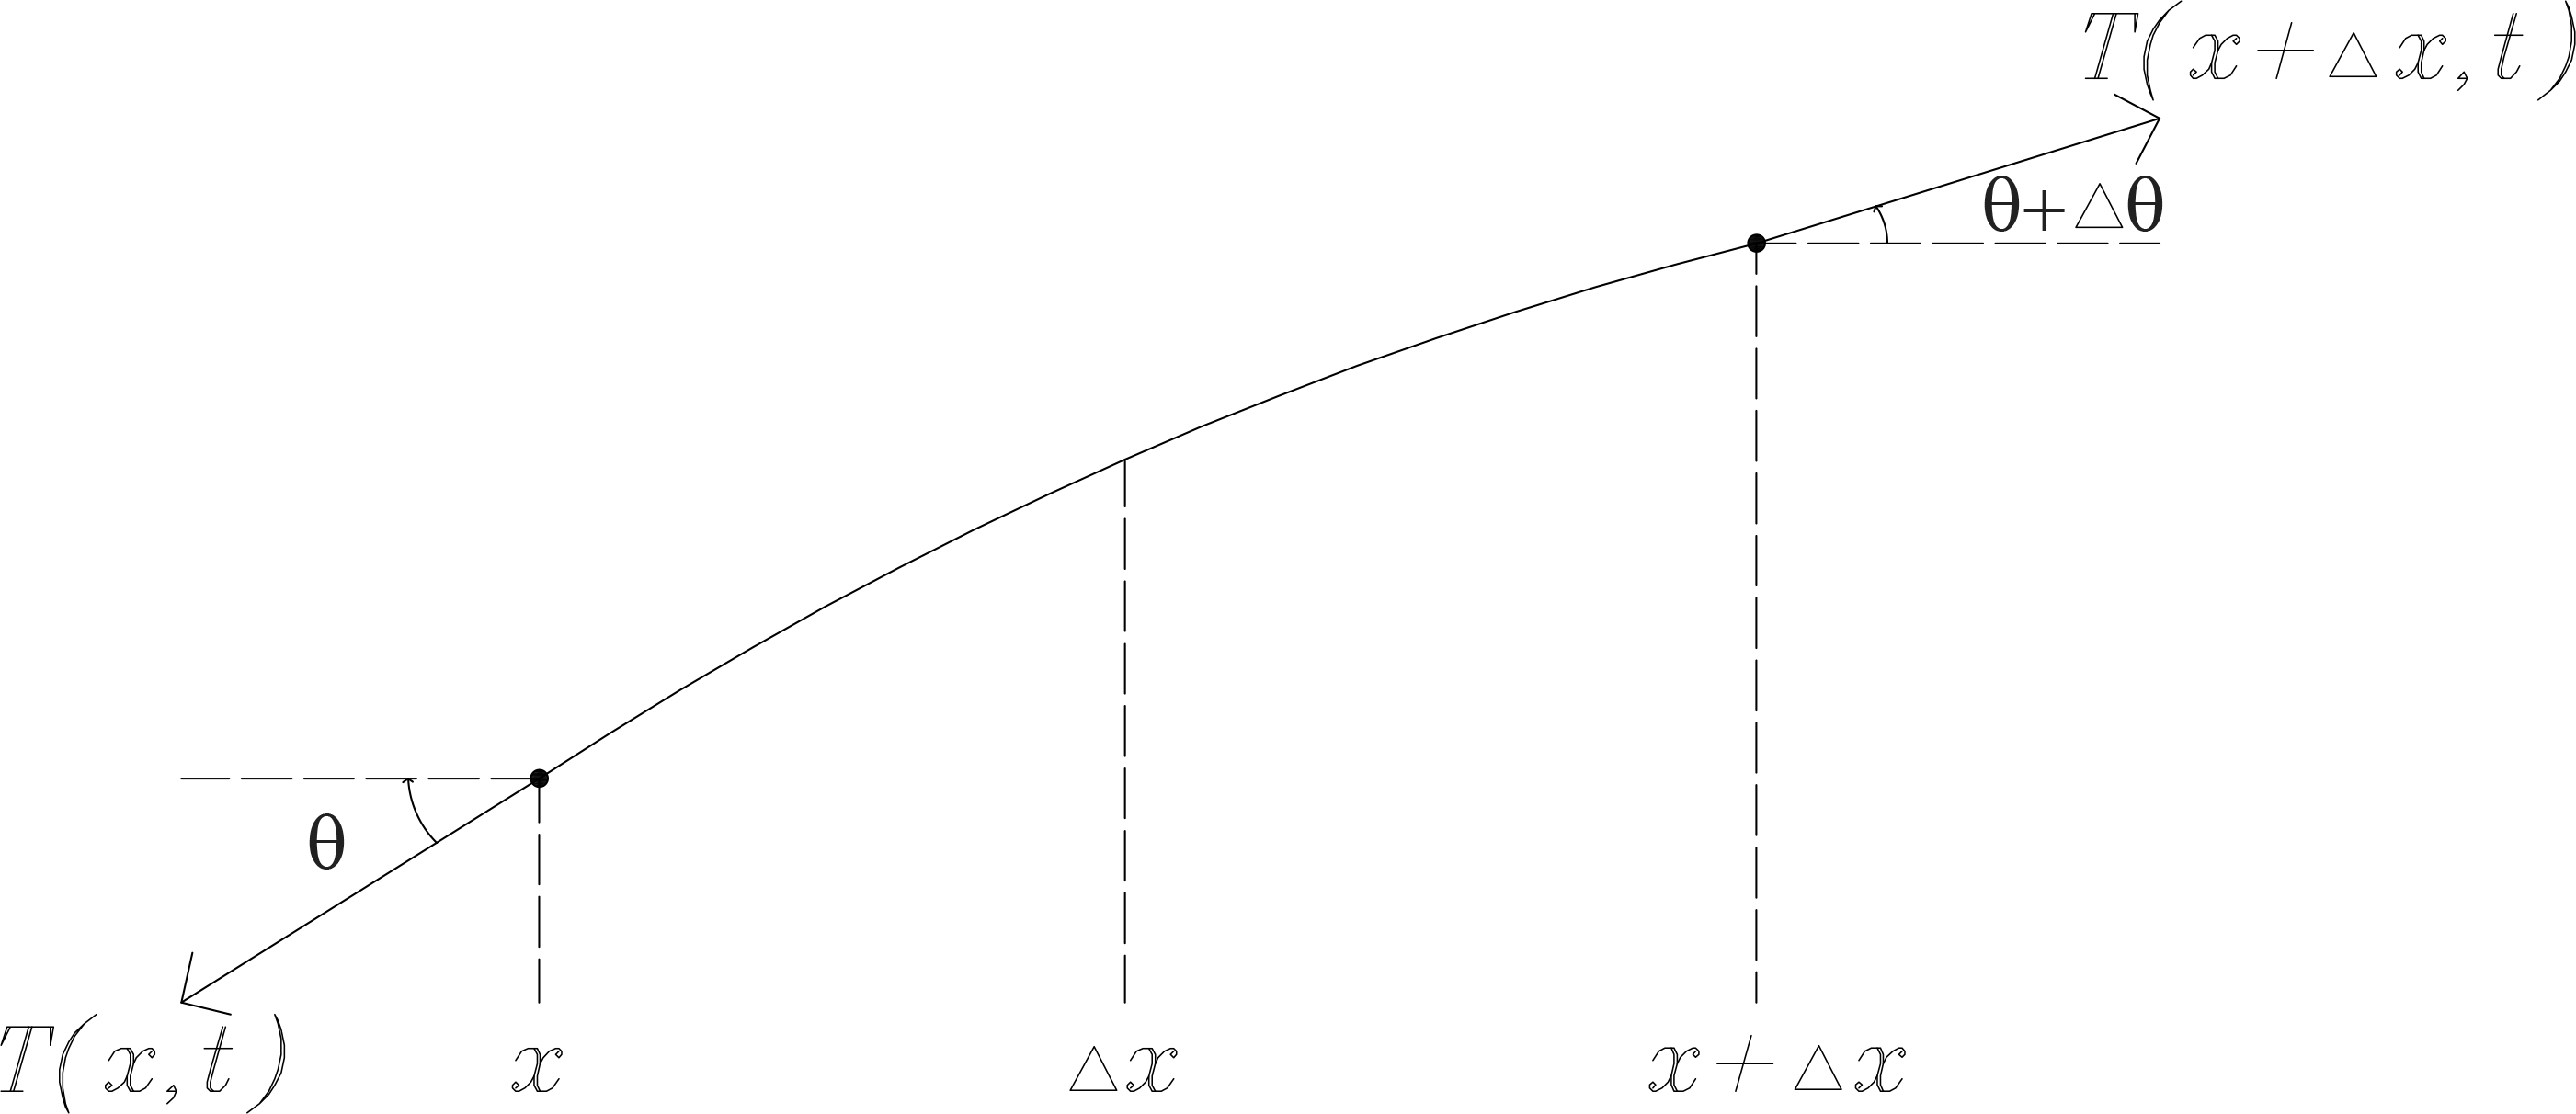
\includegraphics[width=0.9\linewidth]{images/grafic-2.pdf}
        \caption{Components of tension}
        \label{fig:1b}
    \end{subfigure}     
\caption{}
\label{fig:1}
\end{figure}
In \cite[Ch. 1.4]{Tay}, \emph{Newton's Second Law} for a mass that remains
unchanged says that ``for any particle of mass $m$, the net force
$\boldsymbol{F}$ on the particle is always equal to the mass $m$ times the
particle's acceleration: $\boldsymbol{F} = m \boldsymbol{a}$.'' We apply this to
our portion of the string $\Delta x$, so that the external force, the tension at
the ends of the string portion, equals to the product of the mass of the element
and its acceleration at the mass centre. \\

Looking at the movement of the section of string, we see that there is no
acceleration in the horizontal direction, as this movement is insignificant to
the system. Therefore, we obtain the following equation governing the horizontal
motion, by adding together the horizontal components of tension from Figure
\ref{fig:1b}:
\begin {equation} \label{eq1}
    T(x+\Delta x,t)\cos{(\theta + \Delta \theta)}-T(x,t)\cos{\theta}=0
\end {equation}

The left-hand side of (\ref{eq1}) is zero, so this means the whole equation is independent of $x$. For simplification, 
denote the horizontal component of tension by $H: = Tcos\theta$. \\

We now look at the vertical movement and see that there exists a vertical acceleration. This is given by $u_{tt} (\bar{x},t)$, 
where $u_{tt}$ is the second derivative of the displacement with respect to time. Here, $\bar{x}$ is 
the coordinate of the centre of mass of the portion of string and $x<\bar{x}<x+\Delta x$. 
The mass of the section $\Delta x$ is $\rho\Delta x$, and so the vertical movement is given by:
 \begin{equation} \label{eq2}
    T(x+\Delta x,t)\sin{(\theta + \Delta \theta)}-T(x,t)\sin{\theta}=\rho\Delta x u_{tt} (\bar{x},t).
 \end{equation}

 Usually, the weight of the string would also act vertically downwards, but we
 neglect it here. Similarly to the horizontal case, we can denote the vertical
 component of tension by $V=Tcos\theta$ and rewrite (\ref{eq2}) as:
 \begin{equation} \label{eq3}
    \frac{V(x+\Delta x,t)-V(x,t)}{\Delta x}=\rho u_{tt} (\bar{x},t).
 \end{equation}

 Taking the limit of (\ref{eq3}) as $\Delta x \rightarrow 0$ (the equivalent of
 making the string smaller and smaller) we get, from the definition of the
 derivative described in \cite[Ch. 9]{Spi}, that 
 \begin{equation*}
    \lim_{\Delta x \rightarrow 0}\frac{V(x+\Delta x,t)-V(x,t)}{\Delta x}=V_x(x,t),
 \end{equation*}

i.e. that 
\begin {equation} \label{eq4}
    V_x(x,t)=\rho u_{tt} (x,t).
\end{equation}

We want to express equation (\ref{eq4}) in terms of $u$ entirely. Using the
definition of the tangent function we see that the vertical movement is the
horizontal movement multiplied by the tangent: $V(x, t)=H(t)\tan{\theta}$. As the
derivative with respect to $x$ is the slope of the tangent, as in \cite[Ch.
9]{Spi}, we have:
\begin{equation} \label{eq5}
    V(x,t)=H(t)\tan{\theta}=H(t)u_x(x,t).
\end{equation}

Looking back at equation (\ref{eq4}), and combining this with (\ref{eq5}), we
obtain that
\begin{equation*} 
    V_x(x,t)=(H(t)u_x(x,t))_x.
\end{equation*}

Since $H(t)$ is independent of $x$, then this can be written as
$V_x(x,t)=H(t)u_{xx}(x,t)$, which, by equation (\ref{eq4}), gives
\begin {equation} \label{eq7}
    H(t)u_{xx}(x, t)=\rho u_{tt}(x,t).
\end{equation}

Since the motion of the sting is small, we can replace $H=T\cos{\theta}$ by $T$,
as in \cite[Ch. 10, App. B]{BoyDiP}. Hence, (\ref{eq7}) takes the form of the
one-dimensional wave equation:
\begin{equation} \label{wave}
    c^2u_{xx}=u_{tt}, 
\end{equation}
where $c^2=\frac{T}{\rho}$. We can easily verify that $c$ has the dimensions of
velocity, as the tension $T$ is a force and $\rho$ is mass divided by length.

\subsection{Higher Dimensions} \label{twodim}
In the previous section we looked at how to model the string of a musical
instrument, and we obtained the wave equation in one dimension, (\ref{wave}). In
two-dimensions, the elastic string becomes an elastic, flexible and homogeneous
drumhead. The problem is modelled once again using \emph{Newton's Second Law}
for an unchanged mass, to obtain the horizontal and vertical components of
tension. For a full derivation, see \cite[Ch. 12.8]{Kr}. The wave equation in
two dimensions is given by:
\begin{equation} \label{wave2deq13}
    u_{tt}=c^2(u_{xx}+u_{yy}), \quad \textrm{for} \quad x,y \in \mathbb{R}, \quad t \in \mathbb{R}_{>0},
\end{equation}

where, as before, $c^2=\frac{T}{\rho}$, and (\ref{wave2deq13}) can also be
written as $u_{tt}=c^2\Delta u$, where $\Delta u=u_{xx}+u_{yy}$ is the
\emph{Laplacian} of $u$ in two dimensions.\\

We can continue with similar arguments to derive the formula for the
three-dimensional wave equation:
\begin {equation} \label{wave3deq14}
    u_{tt}=c^2(u_{xx}+u_{yy}+u_{zz}), \quad \textrm{for}\quad x,y,z \in \mathbb{R}^3, \quad t \in \mathbb{R}_{>0},
\end{equation}

or $u_{tt}=c^2 \Delta u$ if we use the \emph{Laplacian} in three dimensions.
This equation governs many physical processes and phenomena, such as the
vibration of an elastic solid, sound waves in air, seismic waves propagating
through the Earth, linearised supersonic airflow and electromagnetic waves such
as light and radar, see \cite[Ch. 1, Ex. 3]{Str}. \\

In general, an n-dimensional wave equation has the form $u_{tt}=c^2 \Delta u$,
where $\boldsymbol{x}=(x_1, x_2, ..., x_n)$ is such that $\boldsymbol{x}=(x_1,
x_2, ..., x_n) \in \mathbb{R}^n$ and $t \in \mathbb{R}_{>0}$.

\section{Solution in One Dimension}
In this section, we will prove the D'Alembert solution to the one-dimensional
wave equation (\ref{wave}) in the absence of boundary conditions. The problem we
wish to solve is:
\begin{equation} \label{ivp1d}
    \begin{aligned}
    &u_{tt}-c^2u_{xx}=0, \quad \textrm{for} \quad x\in \mathbb{R},\quad t\in \mathbb{R}_{>0}\\
    &u(x,0)=g(x)\\
    &u_t(x,0)=h(x).
    \end{aligned}
\end{equation}

\subsection{General Form}

We first begin by showing that the solution has the form $u(x,
t)=\phi(\xi)+\psi(\eta)$, where $\xi=x+ct$ and $\eta=x-ct$. This is quite
straightforward as the operator factorises nicely:
\begin{equation} \label{fact1d}
    u_{tt}-c^2u_{xx}=(\diffp[1]{}{t} - c \diffp[1]{}{x})(\diffp[1]{}{t} + c \diffp[1]{}{x})u=0.
\end{equation}

If we denote the second bracket by $v$, we obtain that $v=u_t+cu_x$ and replacing
$v$ into (\ref{fact1d}), we obtain:
\begin{equation*} 
    (\diffp[1]{}{t} -c \diffp[1]{}{x})v=0, \quad \textrm{i.e.} \quad v_t-cv_x=0.
\end{equation*}

We now have two first-order advection equations:
\begin{align}
    v_t-cv_x=0 \label{veq};\\
    u_t+cu_x=v \label{ueq}.
\end{align}

We will focus on solving (\ref{veq}) first. For this, we require a mathematical
technique, the \emph{method of characteristics}, which solves a first-oreder PDE by
converting it into an appropriate system of \emph{ordinary differential equations}
(ODE), see \cite[Ch. 2.1, Ch. 3.2]{Ev}. Variable $v$ is the solution of
(\ref{veq}) and it has the form $v(x(t), t)$. We can use the chain rule to
differentiate $v$ with respect to time:
\begin{equation} \label{diffv}
    \diff{v}{t}=\diffp[1]{v}{t}+\diffp[1]{v}{x}\diff{x}{t}.
\end{equation}

Since $v$ solves both (\ref{veq}) and (\ref{diffv}), we can compare the
equations and see that
\begin{align}
    \diff{v}{t}&=0 \label{xx};\\
    \diff{x}{t}&=-c \label{x}.
\end{align}
The PDE (\ref{veq}) can be regarded as the ODE (\ref{xx}) along any curve
$x(t)$ which is the solution of (\ref{x}). A characteristic curve of our PDE is
a curve given by $x=x(t)$ that satisfies (\ref{x}). From (\ref{xx}) we can see
that the value of $v$ remains constant along such a curve, and therefore, the
solution of (\ref{veq}) has been simplified to the solution of a pair of
simultaneous ODEs: (\ref{xx}) and (\ref{x}). Integrating (\ref{x}), we obtain
the characteristic curves $x(t)=-ct+\alpha$, where $\alpha$ is the intercept of
the curve. At time $t=0$, given by the initial conditions of (\ref{ivp1d}),
$x(0)=\alpha=x_0$, so that $x(t)=-ct+x_0$. Furthermore, with $t-0$, we can let
$v(x,0)=V(x)$, so that the solution of (\ref{veq}) is given by $v(x,t)=V(x+ct)$.
We can verify this is true by differentiating $v$ with respect to $t$ and $x$:
\begin{equation*} 
    \begin{aligned}
    \diffp[1]{}{t}v(x(t), t)=cV'(x+ct)\\
    \diffp[1]{}{x}v(x(t), t)=V'(x+ct),
    \end{aligned}
\end{equation*}

which combined give us precisesly (\ref{veq}), and so $v(x,t)=V(x+ct)$ solves
(\ref{veq}). \\

Next, we want to solve (\ref{ueq}), where $v(x,t)=V(x+ct)$, another advection
equation. Let $w=\diffp[1]{u}{t}-c\diffp{u}{x}$, so that
$\diffp[1]{w}{t}+c\diffp{w}{x}=\diffp[2]{u}{t}-c^2\diffp[2]{u}{x}$. This is is
precisesly the wave equation from (\ref{ivp1d}). This means that, once again, we
have two first-order partial differential equations:
\begin{align}
    \label{weq}
    w_t+cw_x=0\\
    \label{ueqw}
    u_t-cu_x=w.
\end{align}

We solve (\ref{weq}) in a similar manner to (\ref{veq}). If $w(x(t), t)$ solves
(\ref{weq}), then by differentiating $w(x(t),t)$ with respect to time, we obtain:
\begin{equation} \label{diffw}
    \diff{w}{t}=\diffp[1]{w}{t}+\diffp[1]{w}{x}\diff{x}{t}. 
\end{equation}

Comparing (\ref{diffw}) with (\ref{weq}), we get that $\diff{w}{t}=0$ and
$\diff{x}{t}=c$. As before, we want the characteristic curves of this
differential equation. We obtain them by integrating $\diff{x}{t}=c$ to get
$x(t)=ct+x_0$, where $x_0$ is $x$ at time $t=0$. Hence, the solution of
(\ref{weq}) is $w(x,t)=W(x-ct)$. We can verify that this solves the equation by
differentiating. \\

We are now close to the result we set off to prove. Consider $\frac{v+w}{2}$:
\begin{equation*}
    \begin{aligned}
    &\frac{v+w}{2}=\frac{1}{2}\left[\diffp[1]{u}{t}-c\diffp[1]{u}{x}+\diffp[1]{u}{t}+c\diffp[1]{u}{x}\right]=\diffp[1]{u}{t},\\
    &\textrm{i.e.} \quad \diffp[1]{}{t}u(x, t)=\frac{1}{2}\left[V(x+ct)+W(x-ct)\right].
    \end{aligned}
\end{equation*}

When integrating with respect to time, we obtain
\begin{equation} \label{int}
    u(x,t)=\frac{1}{2}\left[\int_0^t{V(x+c\tau)d\tau}+\int_0^t{W(x-c\tau)d\tau}\right].
\end{equation}

The first integral in (\ref{int}) is $\phi(x+ct)$ and the second one is
$\psi(x-ct)$, such that $\phi'=-\frac{1}{2c}V$ and $\psi'=\frac{1}{2c}W$,
respectively. Therefore, the general solution to the one-dimensional wave
equation (\ref{ivp1d}) has the claimed form, 
\begin{equation} \label{gensol}
    u(x, t)=\phi(\xi)+\psi(\eta), \quad \textrm{where} \quad \xi=x+ct \quad \textrm{and} \quad \eta=x-ct.
\end{equation}

\subsection{Initial Value Problem}
We now have the general form (\ref{gensol}) of the solution to the
one-dimensional wave equation from (\ref{ivp1d}). In this section, we will use
it to derive the solution to the initial value problem from (\ref{ivp1d}),
where the initial values are $u(x,0)=g(x)$ and $u_t(x,0)=h(x)$. First, set $t=0$
in (\ref{gensol}). This gives:
\begin{equation} \label{t=0}
    u(x,0)=\phi(x)+\psi(x)=g(x).
\end{equation}

Next, we differentiate (\ref{gensol}) using the chain rule, with respect to $t$
to obtain $u_t(x,t)=c\phi'(x+ct)-c\psi'(x-ct)$. Setting $t=0$ we get:
\begin{equation} \label{ut=0}
    u_t(x,0)=c\phi'(x)-c\psi'(x)=h(x).
\end{equation}

Let $s \in \mathbb{R}$ and differentiate (\ref{t=0}) to obtain:
\begin{equation} \label{eqq9}
    g'(s)=\phi'(s)+\psi'(s).
\end{equation}
Furthermore, divide (\ref{ut=0}) by $c$ to get:
\begin{equation} \label{eqq10}
    \frac{1}{c}h(s)=\phi'(s)-\psi'(s)
\end{equation}
We will continue by adding and subtracting (\ref{eqq9}) and (\ref{eqq10}):
\begin{align} \label{eqq11}
    \phi'(s)=\frac{1}{2}\Big(g'(s)+\frac{1}{c}h(s)\Big),\\
    \label{eqq12}
    \psi'(s)=\frac{1}{2}\Big(g'(s)-\frac{1}{c}h(s)\Big).
\end{align}
Integrating both (\ref{eqq11}) and (\ref{eqq12}) gives:
\begin{align} \label{eqq13}
    \phi(s)=\frac{1}{2}g+\frac{1}{2c}\int^s_0h(\tau)d\tau+A\\
    \label{eqq14}
    \psi(s)=\frac{1}{2}g-\frac{1}{2c}\int^s_0h(\tau)d\tau+B,
\end{align}
where $A$ and $B$ are constants of integration. \\

Equation (\ref{t=0}) tells us that by adding (\ref{eqq13}) and (\ref{eqq14}), we
have $A+B=0$. Substituting $s=x+ct$ for $\phi(s)$ and $s=x-ct$ for $\psi(s)$ we
obtain that
\begin{equation*}
    u(x,t)=\frac{1}{2}g(x+ct)+\frac{1}{2c}\int^{x+ct}_0h(\tau)d\tau+\frac{1}{2}g(x-ct)-\frac{1}{2c}\int^{x-ct}_0h(\tau)d\tau.
\end{equation*}
Rearranging gives the D'Alembert formula to the one-dimensional initial value
wave equation, developed by the mathematician in 1746, see \cite[Ch. 2.1]{Str}:
\begin{equation} \label{DAla}
    u(x,t)=\frac{1}{2}\left[g(x+ct)+g(x-ct)\right]+\frac{1}{2c}\int^{x+ct}_{x-ct}h(\tau)d\tau.
\end{equation}

\subsection{An Application} \label{anapplication}
In this section, we present an application to the one-dimensional
initial value wave equation. We introduce the boundary condition that $u(0,t)=0$
to the problem in (\ref{ivp1d}) and obtain the boundary value problem:
\begin{equation} \label{bvp1d}
    \begin{aligned}
    &u_{tt}-c^2u_{xx}=0 \quad \textrm {for} \quad x \in \mathbb{R}_{\ge 0}, \quad t \in \mathbb{R}_{>0}\\
    &u(x,0)=g(x)\\
    &u_t(x,0)=h(x)\\
    &u(0,t)=0.
    \end{aligned}
\end{equation}

We know how to solve (\ref{ivp1d}), so we will transform (\ref{bvp1d}) into (\ref{ivp1d})
by extending $u,g,h$ to all of $\mathbb{R}$ by odd reflection. See \cite[Ch. 2.4.1]{Ev} for
more details on this method. Hence, we define:
\begin{equation*}
    \begin{aligned}
        &\tilde{u}(x,t):=
        \begin{cases}
            u(x,t) \quad \textrm{when} \quad x \ge 0, t \ge 0\\
            -u(-x,t) \quad \textrm{when} \quad x<0, t \ge 0\\
        \end{cases}
        \\
        &\tilde{g}(x):=
        \begin{cases}
            g(x) \quad \textrm{when} \quad x \ge 0\\
            -g(-x) \quad \textrm{when} \quad x<0\\
        \end{cases}
        \\
        &\tilde{h}(x):=
        \begin{cases}
            h(x) \quad \textrm{when} \quad x \ge 0\\
            -h(-x) \quad \textrm{when} \quad x<0,\\
        \end{cases}
    \end{aligned}
\end{equation*}
and so (\ref{bvp1d}) becomes 
\begin{align*}
    &\tilde{u}_{tt}=c^2\tilde{u}_{xx} \quad \textrm {for} \quad x \in \mathbb{R}, \quad t \in \mathbb{R}_{>0} \\
    &\tilde{u}(x,0)=\tilde{g}(x)\\
    &\tilde{u}_t(x,0)=\tilde{h}(x).\\
\end{align*}
This looks exactly like (\ref{ivp1d}), so we can use the D'Alembert formula
(\ref{DAla}) to find a solution for $\tilde{u}$:
\begin{equation*}
    \tilde{u}(x,t)=\frac{1}{2}\left[\tilde{g}(x+ct)+\tilde{g}(x-ct)\right]+\frac{1}{2c}\int^{x+ct}_{x-ct}\tilde{h}(\tau)d\tau.
\end{equation*}

Recalling the definitions of $\tilde{u}, \tilde{g}$ and $\tilde{h}$ gives us the
solution to (\ref{bvp1d}):
\begin{equation} \label{bvpsol}
    u(x,t)=
    \begin{cases}
        \frac{1}{2}\left[g(x+ct)+g(x-ct)\right]+\frac{1}{2c}\int^{x+ct}_{x-ct}h(\tau)d\tau \quad \textrm{if} \quad x \ge ct \ge 0\\
        \frac{1}{2}\left[g(x+ct)-g(ct-x)\right]+\frac{1}{2c}\int^{x+ct}_{-x+ct}h(\tau)d\tau \quad \textrm{if} \quad 0 \le x \le ct\\
    \end{cases}
\end{equation}

We will use the solution (\ref{bvpsol}) to the boundary value wave equation
(\ref{bvp1d}) to solve the three-dimensional wave equation in the next section.
Note that if $h \equiv 0$, then (\ref{bvpsol}) can be understood as a split in
the initial displacement, one moving to the right, and one to the left, see
\cite[Ch. 2.4.1]{Ev}. Furthermore, this solution does not belong to $C^2$, the set of twice
differentiable functions, unless $g''(0)=0$.

\section{Solution in Three Dimensions} \label{sec3d}
In this section, we will derive the solution to the three-dimensional wave
equation (\ref{wave3deq14}), as described in \cite[Chap. 2.4]{Ev}. To do this,
we will use \emph{spherical means}, which allow us to transform the partial
differential equation into an integral over a sphere of radius $r$, centred at
some point $\boldsymbol{x}$. For more information on spherical means, please
see \cite{Sab}.
\\

The problem we wish to solve is
\begin{equation} \label{3deq}
\begin{aligned}
    &u_{tt}-c^2(u_{xx}+u_{yy}+u_{zz})=0 \quad \textrm {for} \quad x, y, z \in \mathbb{R}, \quad t \in \mathbb{R}_{>0}\\
    &u(x, y, z,0)=g(x,y,z)\\
    &u_t(x,y,z,0)=h(x,y,z).\\
\end{aligned}
\end{equation}

We intend, in this section, to derive the formula for $u$ in terms of $g$ and
$h$. We plan to look at the average of $u$ as a function of the time and radius
over certain spheres, and apply the D'Alembert formula (\ref{bvpsol}) from
Section \ref{anapplication}. Note that throughout the next sections, we will let
$\boldsymbol{x}=(x,y,z)$.

\subsection{Some Prerequisite Results} \label{prereq}
As we proceed with our derivation of the three-dimensional wave equation, we require
some other results, which we will not prove. \\

Firstly, we introduce some notation to simplify our work in the upcoming
sections. Let $u$ be the solution of (\ref{3deq}). If we let $\boldsymbol{x}\in \mathbb{R}^n, t>0, r>0$, then we have:

\begin{equation} \label{averageU}
    U(\boldsymbol{x};r,t)=\dashint_{\partial B(\boldsymbol{x},r)}u(\boldsymbol{y},t)dS(\boldsymbol{y}),
\end{equation}

the average of $u(\cdot,t)$ over the sphere $\partial B(\boldsymbol{x},r)$, where
$dS(\boldsymbol{y})$ is the three-dimensional surface measure on $\partial B(\boldsymbol{x},r)$,
as in \cite[Ch. 2.4.1 b]{Ev}. Similarly, we have the averages of $g$ and $h$ over the same
sphere:
\begin{equation} \label{averageGH}
    \begin{aligned}
        &G(\boldsymbol{x},r)=\dashint_{\partial B(\boldsymbol{x},r)}g(\boldsymbol{y})dS(\boldsymbol{y})\\
        &H(\boldsymbol{x},r)=\dashint_{\partial B(\boldsymbol{x},r)}h(\boldsymbol{y})dS(\boldsymbol{y}).
    \end{aligned}
\end{equation}

When we fix $\boldsymbol{x}$, we can regard $U$ as a function of just $r$ and
$t$. Note that if $u$ satisfies equation (\ref{3deq}), then we have $U \in
C^m(\mathbb{R}_{\ge 0}\times[0,\infty))$, where $\mathbb{R}_{\ge 0}$ is the set
of all the positive real numbers, and $m \ge 2$. Then $U$ satisfies the \emph{Euler-Poisson-Darboux equation}:
\begin{equation} \label{EPDeq}
    \begin{aligned}
        &U_{tt}-c^2U_{rr}-c^2\frac{n-1}{r}U_r=0 \quad \textrm {for} \quad r \in \mathbb{R}_{>0}, \quad t \in \mathbb{R}_{>0}, \quad n \ge 2\\
        &U(r, 0)=G(r)\\
        &U_t(r,0)=H(r).
    \end{aligned}
\end{equation}
\\

Another piece of mathematics we require for our derivation of the solution of
the three-dimensional wave equation is the transformation formula for surface
integrals. That is, we want to show $\int_{\partial
B(\boldsymbol{x},t)}f(\boldsymbol{y})dS=r^2\int_{\partial B(\boldsymbol{0},1)}
f(\boldsymbol{x}+r\boldsymbol{z})dS(\boldsymbol{z})$. Let $y:U \rightarrow
\partial B(\boldsymbol{x}, r)$, where $U \subseteq \mathbb{R}^3$ is open. The change of variables
formula in $\mathbb{R}^3$ from \cite[Ch. 11, Th. 11.1]{LooSter} gives:
\begin{equation*}
    \int_{\partial B(\boldsymbol{x},r)}f(\boldsymbol{y})dS(y)=\int_U f(\boldsymbol{y}(s,t))\left\| \diffp[1]{}{s}\boldsymbol{y}(s, t) \times \diffp[1]{}{t}\boldsymbol{y}(s, t) \right \|ds dt
\end{equation*}

The function $f(\boldsymbol{y})$ can be written as
$f(\boldsymbol{y})=f(\boldsymbol{x}+r(\frac{\boldsymbol{y}-\boldsymbol{x}}{r}))$
such that $\boldsymbol{y}(s,t)$ can be thought of as a parametrisation of any
sphere $\partial B(\boldsymbol{x},r)$ for $(s,t)\in U$. Then we can see that
$\frac{\boldsymbol{y}(s,t)-\boldsymbol{x}}{r}$ is a parametrisation of the
sphere of radius 1, centred at the origin, $\partial B(\boldsymbol{0},1)$ for
the same $(s,t)\in U$. Furthermore, using these parametrisations, we obtain
\begin{equation*}
    \left \| \diffp[1]{\boldsymbol{y}}{s} \times \diffp[1]{\boldsymbol{y}}{t} \right \| =r^2 \left \| \diffp[1]{}{s}\Big(\frac{\boldsymbol{y}-\boldsymbol{x}}{r}\Big) \times \diffp[1]{}{s}\Big( \frac{\boldsymbol{y}-\boldsymbol{x}}{r}\Big) \right \|.
\end{equation*}

Letting $\boldsymbol{z}(s,t)=\frac{\boldsymbol{y}(s,t)-\boldsymbol{x}}{r}$, we
obtain our required result:
\begin{equation*}
    \begin{aligned}
    \int_U f(\boldsymbol{y}(s,t)) \left \| \diffp[1]{}{s}\boldsymbol{y}(s, t) \times \diffp{}{t}\boldsymbol{y}(s, t) \right \| dsdt&=r^2\int_U f(\boldsymbol{x}+r\boldsymbol{z}(s,t)) \left \| \diffp[1]{}{s}\boldsymbol{z}(s, t) \times \diffp[1]{}{t}\boldsymbol{z}(s, t) \right \| dsdt\\
    &=r^2\int_{\partial B(\boldsymbol{0},1)}f(\boldsymbol{x}+r\boldsymbol{z})dS(\boldsymbol{z}).
    \end{aligned}
\end{equation*}

\subsection{Kirchhoff's Formula}
We now want to derive the formula for the solution to the wave equation in
three-dimensions (\ref{3deq}), following the method presented in \cite[Ch. 2.4.1.c]{Ev}. We will assume that $u \in C^2(\mathbb{R}^3
\times [0, \infty))$ solves (\ref{3deq}). Let us denote:
\begin{equation} \label{Udash}
    \tilde{U}:=rU
\end{equation}
\begin{equation} \label{GHdash}
    \begin{aligned}
        &\tilde{G}:=rG\\
        &\tilde{H}:=rH,    
    \end{aligned}
\end{equation}

where $U,G$ and $H$ are defined as in (\ref{averageU}) and (\ref{averageGH}),
respectively. \\

As $U$ solves the \emph{Euler-Poisson-Darboux equation}, (\ref{EPDeq}), we can
use he notation of (\ref{Udash}) and (\ref{GHdash}) to obtain the boundary value
problem solved in Section \ref{anapplication}:

\begin{equation*}
    \begin{aligned}
        \tilde{U}_{tt}&=rU_{tt}\\
        &=r\Big[c^2U_{rr}+c^2\frac{2}{r}U_r\Big] \quad \textrm{by (\ref{EPDeq}) with} \quad n=3\\
        &=c^2rU_{rr}+2c^2U_r\\
        &=c^2(rU_{rr}+2U_r)\\
        &=c^2(U+rU_r)_r\\
        &=c^2(rU)_{rr}\\
        &=c^2\tilde{U}_{rr}.        
    \end{aligned}
\end{equation*}

This means that $\tilde{U}$ solves:
\begin{equation} \label{tilUwave}
    \begin{aligned}
        &\tilde{U}_{tt}-c^2\tilde{U}_{rr}=0 \quad \textrm {for} \quad r \in \mathbb{R}, \quad t \in \mathbb{R}_{>0}\\
        &\tilde{U}(r, 0)=\tilde{G}(r) \\
        &\tilde{U}_t(r, 0)=\tilde{H}(r)\\
        &\tilde{U}(0, t)=0.
    \end{aligned}
\end{equation}

Note that $\tilde{G}_{rr}(0)=0$ as $\tilde{U}(r,0)=\tilde{G}(r)$ in
(\ref{tilUwave}). As this boundary value problem is the same as (\ref{bvp1d}),
then we can apply the solution (\ref{bvpsol}) to (\ref{tilUwave}). Hence, for $0
\le r \le ct$ we have 
\begin{equation} \label{newUtil}
    \tilde{U}(\boldsymbol{x};r,t)=\frac{1}{2}\left[\tilde{G}(r+ct)-\tilde{G}(ct-r)\right]+\frac{1}{2c}\int^{r+ct}_{-r+ct}\tilde{H}(\boldsymbol{y})d\boldsymbol{y}.
\end{equation} 

Our definition of $U$ from (\ref{averageU}) implies that
 $u(\boldsymbol{x},t)=\lim_{r\rightarrow 0^+}U(\boldsymbol{x};r,t)$,see
 \cite[Ch. 2.4.1.c]{Ev} so our definitions of $\tilde{G}, \tilde{H}$ in
 (\ref{GHdash}), and the new expression for $\tilde{U}$ from (\ref{newUtil})
 lead to:
\begin{equation} \label{almostK}
    \begin{aligned}
        u(\boldsymbol{x},t)&=\lim_{r\rightarrow 0^+}\frac{\tilde{U}(\boldsymbol{x};r,t)}{r}\\
        &=\lim_{r\rightarrow 0^+}\left[\frac{\tilde{G}(r+ct)-\tilde{G}(ct-r)}{2r}+\frac{1}{2rc}\int^{r+ct}_{-r+ct}\tilde{H}(\boldsymbol{y})d\boldsymbol{y}\right]\\
        &=\tilde{G}'(ct)+\frac{1}{c}\tilde{H}(ct)\\
        &=\diffp[1]{}{t}\Big[t\dashint_{\partial B(\boldsymbol{x},t)}{gdS} \Big]+\frac{t}{c}\dashint_{\partial B(\boldsymbol{x},t)}{hdS} \quad \textrm{by (\ref{averageGH})}
    \end{aligned}
\end{equation}

In section \ref{prereq} we saw that $\int_{\partial
B(\boldsymbol{x},t)}f(\boldsymbol{y})dS=r^2\int_{\partial B(\boldsymbol{0},1)}
f(\boldsymbol{x}+t\boldsymbol{z})dS(\boldsymbol{z})$. Looking at the averages
notation, then for sufficiently smooth $f$ we have $\dashint_{\partial
B(\boldsymbol{x}, t)} f(\boldsymbol{y})dS(\boldsymbol{y}) = \dashint_{\partial
B(\boldsymbol{0}, 1)} f(\boldsymbol{x}+t\boldsymbol{z})dS(\boldsymbol{z})$. We
will use this to complete our solution of the three-dimensional wave equation:
\begin{equation*}
    \begin{aligned}
    t\diffp[1]{}{t}\dashint_{\partial B(\boldsymbol{x},t)} {g(\boldsymbol{y})dS(\boldsymbol{y})} &= \diffp[1]{}{t} t \dashint_{\partial B(\boldsymbol{0}, 1)}g(\boldsymbol{x}+t\boldsymbol{z})dS(\boldsymbol{z})\\
    &=\dashint_{\partial B(\boldsymbol{0}, 1)}g(\boldsymbol{x}+t\boldsymbol{z})dS(\boldsymbol{z}) + t \dashint_{\partial B(0,1)} {Dg(\boldsymbol{x}+t\boldsymbol{z})\cdot \boldsymbol{z}dS(\boldsymbol{z})}\\
    &=\dashint_{\partial B(\boldsymbol{x},t)} {g(\boldsymbol{y})dS(\boldsymbol{y})}+t \dashint_{\partial B(\boldsymbol{x},t)}{Dg(\boldsymbol{y})(\frac{\boldsymbol{y}-\boldsymbol{x}}{t})dS(\boldsymbol{y})}\\
    &=\dashint_{\partial B(\boldsymbol{x},t)} {g(\boldsymbol{y})dS(\boldsymbol{y})}+\dashint_{\partial B(\boldsymbol{x},t)}{Dg(\boldsymbol{y})(\boldsymbol{y}-\boldsymbol{x})dS(\boldsymbol{y})},
    \end{aligned}
\end{equation*}

where $D$ represents the first-order derivative with respect to time.
Substituting this into (\ref{almostK}), we obtain the solution to the
three-dimensional wave equation, which is known as \emph{Kirchhoff's formula},
but is actually, due to Poisson, see \cite[Ch. 9.2]{Str}:
\begin{equation} \label{KircE}
    u(\boldsymbol{x},t)=\frac{1}{c^2}\dashint_{\partial B(\boldsymbol{x},t)} (th(\boldsymbol{y})+Dg(\boldsymbol{y})(\boldsymbol{y}-\boldsymbol{x})+g(\boldsymbol{y}))dS(\boldsymbol{y}).
\end{equation}

\subsection{Another Formula}
\emph{Strauss}, in \cite[Ch. 9.2]{Str} gives another form of Kirchhoff's formula for the
solution to the wave equation in three-dimensions. In this section, we aim to
prove that this formula is the same as the one we have seen in (\ref{KircE}).
The formulation mentioned in \cite[Ch. 9.2]{Str} is as follows, where
$\boldsymbol{x}=(x,y,z)$, as before:
\begin{equation} \label{KircSTR}
    u_S(\boldsymbol{x}, t)=\frac{1}{4 \pi c^2 t}\iint_{\partial B(\boldsymbol{x}, t)}h(\boldsymbol{y})dS(\boldsymbol{y})+\diffp[1]{}{t}\Big( \frac{1}{4 \pi c^2 t}\iint_{\partial B(\boldsymbol{x}, t)} g(\boldsymbol{y})\Big)dS(\boldsymbol{y}).
\end{equation}

For a more comfortable identification of the two formulae by different authors,
we will rewrite (\ref{KircE}): 
\begin{equation} \label{KircEV}
    u_E(\boldsymbol{x},t)=\frac{1}{c^2}\dashint_{\partial B(\boldsymbol{x},t)}(th(\boldsymbol{y})+Dg(\boldsymbol{y})(\boldsymbol{y}-\boldsymbol{x})+g(\boldsymbol{y}))dS(\boldsymbol{y}).
\end{equation}

In order to start identifying common parts between the two formulae, recall that
$\dashint_{\partial B(\boldsymbol{x}, t)}$ was the average over the sphere
$\partial B(\boldsymbol{x}, t)$. This is the same as $\frac{1}{4 \pi
t^2}\iint_{\partial B(\boldsymbol{x}, t)}$, since the surface area of the sphere
is $4\pi r^2$, where $r$ is the radius of the sphere, in our case, $t$. Using
this, we can rewrite (\ref{KircEV}) as:
\begin{equation*}
    \begin{aligned}
    u_E(\boldsymbol{x},t)&=\frac{1}{4 \pi c^2 t^2}\iint_{\partial B(\boldsymbol{x},t)} (th(\boldsymbol{y})+Dg(\boldsymbol{y})(\boldsymbol{y}-\boldsymbol{x})+g(\boldsymbol{y}))dS(\boldsymbol{y})\\ 
    &=\frac{1}{4 \pi c^2 t^2}\iint_{\partial B(\boldsymbol{x},t)} th(\boldsymbol{y})dS(\boldsymbol{y})+\frac{1}{4 \pi c^2 t^2}\iint_{\partial B(\boldsymbol{x},t)}(Dg(\boldsymbol{y})(\boldsymbol{y}-\boldsymbol{x})+g(\boldsymbol{y}))dS(\boldsymbol{y}).
    \end{aligned}
\end{equation*}

Our aim is to show that $u_S$ and $u_E$ are the same. We start by letting $g=0$
in both (\ref{KircEV}) and (\ref{KircSTR}):
\begin{equation} \label{g=0}
    \begin{aligned}
        u_S(\boldsymbol{x}, t)&=\frac{1}{4\pi c^2 t}\iint_{\partial B(\boldsymbol{x}, t)}h(\boldsymbol{y})dS(\boldsymbol{y})\\
        &=\frac{1}{4\pi c^2 t^2}\iint_{\partial B(\boldsymbol{x}, t)}th(\boldsymbol{y})dS(\boldsymbol{y})\\
        &=u_E(\boldsymbol{x}, t).
    \end{aligned}
\end{equation}

This computation shows that the first parts of the two formulae are the same.
Next, we show that the second parts are the same by letting $h=0$:
\begin{equation} \label{starr}
    \begin{aligned}
        u_S(\boldsymbol{x},t)&=\diffp[1]{}{t}\frac{1}{4\pi c^2 t}\iint_{\partial B(\boldsymbol{x}, t)}g(\boldsymbol{y})dS(\boldsymbol{y})\\
        &=\diffp[1]{}{t}t\Big(\frac{1}{4\pi c^2 t^2}\iint_{\partial B(\boldsymbol{x}, t)}g(\boldsymbol{y})dS(\boldsymbol{y})\Big)\\
        &=\frac{1}{c^2}\diffp[1]{}{t}t\Big(\dashint_{\partial B(\boldsymbol{x}, t)}g(\boldsymbol{y})dS(\boldsymbol{y})\Big).
    \end{aligned}
\end{equation}

Using the transformation of surface integrals described in section \ref{prereq},
we obtain that $\dashint_{\partial B(\boldsymbol{x},
t)}g(\boldsymbol{y})dS(\boldsymbol{y})=\dashint_{\partial B(\boldsymbol{0},
1)}g(\boldsymbol{x}+t\boldsymbol{z})dS(\boldsymbol{z})$. This means that
(\ref{starr}) becomes:
\begin{equation} \label{h=0} 
    \begin{aligned}
        u_S(\boldsymbol{x}, t)&=\frac{1}{c^2}\diffp[1]{}{t}t\Big(\dashint_{\partial B(\boldsymbol{0}, 1)}g(\boldsymbol{x}+t\boldsymbol{z})dS(\boldsymbol{z})\Big)\\
        &=\frac{1}{c^2}\dashint_{\partial B(\boldsymbol{0}, 1)}g(\boldsymbol{x}+\frac{1}{c^2}t\boldsymbol{z})dS(\boldsymbol{z})+t\diffp[1]{}{t}\dashint_{\partial B(\boldsymbol{0}, 1)}g(\boldsymbol{x}+t\boldsymbol{z})dS(\boldsymbol{z})\\
        &=\frac{1}{c^2}\dashint_{\partial B(\boldsymbol{0}, 1)}g(\boldsymbol{x}+\frac{1}{c^2}t\boldsymbol{z})dS(\boldsymbol{z})+t\dashint_{\partial B(\boldsymbol{0}, 1)}Dg(\boldsymbol{x}+t\boldsymbol{z}) \cdot \boldsymbol{z}dS(\boldsymbol{z})\\
        &=\frac{1}{c^2}\dashint_{\partial B(\boldsymbol{x}, t)}g(\boldsymbol{y})dS(\boldsymbol{y})+\frac{1}{c^2}t\dashint_{\partial B(\boldsymbol{x}, t)}Dg(\boldsymbol{y})\Big(\frac{\boldsymbol{y}-\boldsymbol{x}}{t}\Big)dS(\boldsymbol{y})\\
        &=\frac{1}{c^2}\dashint_{\partial B(\boldsymbol{x}, t)}g(\boldsymbol{y})dS(\boldsymbol{y})+\frac{1}{c^2}t\dashint_{\partial B(\boldsymbol{x}, t)}Dg(\boldsymbol{y})(\boldsymbol{y}-\boldsymbol{x})dS(\boldsymbol{y})\\
        &=u_E(\boldsymbol{x},t).
    \end{aligned}
\end{equation}

Since in both (\ref{g=0}) and (\ref{h=0}) we showed that $u_S=u_E$, then we can
conclude that the two solutions to the three-dimensional wave equation are the
same.

\section{Solution in Two-Dimensions} \label{sec2d}
In this section, we will present the solution to the two-dimensional wave
equation presented in  Section \ref{twodim}. Before we prove the solution, we will discuss
\emph{Huygens' Principle} and explain why we solved the three-dimensional
equation first.

\subsection{Huygens' Principle}
\emph{Huygens' Principle} describes how we can physically hear sharp sounds and
see sharp images. \emph{Folland}, in \cite[Ch 5.B]{Fol}, gives a very simple
example to illustrate this. If we are in a dark room at a position $x_0$ that
doesn't change, and we set off a flash light at the origin of the
three-dimensional system we created from the room, at time $t=0$, then we will
be able to see the light only for as long as it takes it to travel from its
position to where we are, the room becoming dark again after. Another simple
example to illustrate \emph{Huygens' Principle} is given by \emph{Strauss} in
\cite[Ch. 9.2]{Str}, where he looks at how the sound of a musical instrument is
heard by the human ear. Sound is carried through air at precisely the fixed
speed $c$ without any disturbance by assuming there are no walls or other
inhomogeneities in the air.Then at any time $t$, the listener hears exactly what
notes the musical instrument plays at the time $t-\frac{d}{c}$, where $d$ is the
distance between the listener and the instrument, rather than hearing a mixture
of notes from earlier echoing over the new notes. These three-dimensional
examples show phenomena that are described by \emph{Huygens' Principle}, which
asserts that an initial state is observed at a different place as an effect that
is very rigorously delimited, see \cite[Ch. III, \S 4.6]{Hil} . \\

This physical phenomenon makes sense in three-dimensions, and it is encountered
in everyday life. However, we are also interested in what happens if a
two-dimensional system would follow the same rules. This does not make sense,
and an example to show this comes from dropping a pebble into an undisturbed
pond. The waves that are created by the pebble satisfy approximately well the
two-dimensional wave equation with a certain speed $c$, where $x$ and $y$ are
horizontal coordinates of the 2D plane. If we assume there exists a waterbug
without any movement, at a distance $d$ from the point of impact between the
pebble and the water, it will feel a wave at time $t=\frac{d}{c}$, but that wave
will not stop upon reaching the waterbug but continue to send out waves. Those
secondary waves become so small that they are no longer felt after a period of
time, but they do not actually ever stop, see \cite[Ch. 9.2]{Str}. This means
that \emph{Huygens' Principle} no longer holds. This is because the time does
not limit the initial state, i.e. once a signal reaches a point in the
two-dimensional space, it continues there indefinitely. More details about the
physical interpretations can be found in \cite[Ch. III, \S 4.6]{Hil}. \\

\emph{Huygens's Principle} allowed us to straightforwardly derive the solution
of the three-dimensional equation using spherical means. However, this same
principle means that the same method cannot be employed to solve the
two-dimensional equation, but it offers an alternative based on the
three-dimensional problem. The trick is to solve the case in three dimensions
and then \emph{descend} into two dimensions by letting the $z$-coordinate in
$u_{tt}=c^2(u_{xx}+u_{yy}+u_{zz})$ equal $0$, as in \cite[Ch. 2.4.1.c]{Ev}. We shall see how
this works in the next section. 

\subsection{Poisson's Formula}

In this section, we will prove the solution to the two-dimensional wave
equation. We cannot transform the \emph{Euler-Poisson-Darboux equation}
(\ref{EPDeq}) using (\ref{Udash}) and (\ref{GHdash}) into the one-dimensional
equation when $n=2$. This is why we do not have a specific method to solving the
two-dimensional problem other than considering it as the previously solved
three-dimensional problem with the third spatial coordinate equal to $0$. Let
the function $u(\boldsymbol{x},t) \in C^2(\mathbb{R}^2 \times [0, \infty))$
solve the wave equation in two dimensions:
\begin{equation} \label{2d}
    \begin{aligned}
        &u_{tt}-c^2(u_{xx}+u_{yy})=0 \quad \textrm{with} \quad x,y \in \mathbb{R}, \quad t\in \mathbb{R}_{>0}\\
        &u(x, y, 0)=g(x,y),\\
        &u_t(x,y,0)=h(x,y).
    \end{aligned}
\end{equation}

Then, we can let $\bar{u}(x, y, z, t):=u(x, y, t)$ such that the problem we wish
to solve becomes:
\begin{equation} \label{2das3d}
    \begin{aligned}
        &\bar{u}_{tt}-c^2(\bar{u}_{xx}+\bar{u}_{yy}+\bar{u}_{zz})=0 \quad \textrm{with} \quad x,y,z \in \mathbb{R}, \quad t\in \mathbb{R}_{>0}\\
        &\bar{u}(x, y, z, 0)=\bar{g}(x,y,z), \quad \textrm{where} \quad \bar{g}(x,y,z)=g(x,y)\\
        &\bar{u}_t(x,y,z,0)=\bar{h}(x,y,z), \quad \textrm{where} \quad \bar{h}(x,y,z)=h(x,y).
    \end{aligned}
\end{equation}

Let $\boldsymbol{x}=(x,y)\in \mathbb{R}^2$ and $\boldsymbol{\bar{x}}=(x,y, 0)\in
\mathbb{R}^3$. Then, combining (\ref{2das3d}) with the (\ref{almostK}) form of
Kirchhoff's formula, we obtain:
\begin{equation} \label{star}
    \begin{aligned}
        u(\boldsymbol{x},t)&=\bar{u}(\boldsymbol{\bar{x}}, t)\\
        &=\diffp[1]{}{t}\Big(t\dashint_{\partial \bar{B}(\boldsymbol{\bar{x}}, t)} \bar{g}(\boldsymbol{y}) d\bar{S}(\boldsymbol{y}\Big)+\frac{t}{c} \dashint_{\partial \bar{B}(\boldsymbol{\bar{x}}, t)} \bar{h}(\boldsymbol{y})d\bar{S}(\boldsymbol{y}),
    \end{aligned}
\end{equation}

where $\partial\bar{B}(\boldsymbol{\bar{x}},t)$ is the ball centered at
$\boldsymbol{\bar{x}}$, of radius $t>0$, in $\mathbb{R}^3$, and that $d\bar{S}$
is the two-dimensional measure on $\partial\bar{B}(\boldsymbol{\bar{x}},t)$.
Note that $\dashint_{\partial \bar{B}(\boldsymbol{\bar{x}}, t)}
\bar{g}(\boldsymbol{y}) d\bar{S}(\boldsymbol{y})=\frac{1}{4\pi
t^2}\int_{\partial \bar{B}(\boldsymbol{\bar{x}}, t)}\bar{g} (\boldsymbol{y})
d\bar{S} (\boldsymbol{y})$, as they both represent the average over the sphere.
Let $\gamma (\boldsymbol{y})=(c^2 t^2-|\boldsymbol{y}-\boldsymbol{x}|^2)^{1/2}$,
for $\boldsymbol{y} \in B(\boldsymbol{x}, t)$. Let $\boldsymbol{y} \in
B(\boldsymbol{x}, t)$ because in two dimensions, we no longer have a sphere, but
a ball of radius $t$, centered at $\boldsymbol{x}$. Using this we obtain:
\begin{equation} \label{tired}
    \begin{aligned}
        \dashint_{\partial \bar{B}(\boldsymbol{\bar{x}}, t)} \bar{g} d\bar{S}&=\frac{1}{4\pi t^2}\int_{\partial \bar{B}(\boldsymbol{\bar{x}}, t)}\bar{g} d\bar{S}\\
        &=\frac{2}{4 \pi t^2} \int_{B(\boldsymbol{x}, t)} g(\boldsymbol{y})(1+|D\gamma (\boldsymbol{y})|^2)^{1/2}d\boldsymbol{y}.
    \end{aligned}
\end{equation}

We have $2$ as the numerator of the fraction as the sphere
$\partial\bar{B}(\boldsymbol{\bar{x}}, t)$ consists of two hemispheres.
Furthermore, $D\gamma (\boldsymbol{y})$ is the first derivative of $\gamma$ with
respect to $\boldsymbol{y}$, and it is $D\gamma
(\boldsymbol{y})=-\frac{|\boldsymbol{y}-\boldsymbol{x}|}{(c^2
t^2-|\boldsymbol{y}-\boldsymbol{x}|^2)^{1/2}}$. Then,
\begin{equation*}
    \begin{aligned}
        (1+|D\gamma (\boldsymbol{y})|^2)^{1/2}&=\Big(1+\Big(\frac{|\boldsymbol{y}-\boldsymbol{x}|}{(c^2 t^2-|\boldsymbol{y}-\boldsymbol{x}|^2)^{1/2}}\Big)^2\Big)^{1/2}\\
        &=\Big(1+\frac{|\boldsymbol{y}-\boldsymbol{x}|^2}{c^2 t^2-|\boldsymbol{y}-\boldsymbol{x}|^2}\Big)^{1/2}\\
        &=\Big(\frac{t^2}{c^2 t^2-|\boldsymbol{y}-\boldsymbol{x}|^2}\Big)^{1/2}\\
        &=t(c^2 t^2-|\boldsymbol{y}-\boldsymbol{x}|^2)^{-1/2}.
    \end{aligned}
\end{equation*}

So, our integral (\ref{tired}) becomes:
\begin{equation*}
    \begin{aligned}
        \dashint_{\partial \bar{B}(\boldsymbol{\bar{x}}, t)} \bar{g}(\boldsymbol{y}) d\bar{S}(\boldsymbol{y})&=\frac{1}{2 \pi t^2}\int_{B(\boldsymbol{x},t)}\frac{tg(\boldsymbol{y})}{(c^2 t^2-|\boldsymbol{y}-\boldsymbol{x}|^2)^{1/2}}d\boldsymbol{y}\\
        &=\frac{1}{2 \pi t}\int_{B(\boldsymbol{x},t)}\frac{g(\boldsymbol{y})}{(c^2 t^2-|\boldsymbol{y}-\boldsymbol{x}|^2)^{1/2}}d\boldsymbol{y}.
    \end{aligned}
\end{equation*}

Hence, (\ref{star}) is: 
\begin{equation*}
    \begin{aligned}
        u(\boldsymbol{x},t)&=\diffp[1]{}{t}\Big(t \frac{1}{4 \pi t^2} \int_{\partial \bar{B}(\boldsymbol{\bar{x}}, t)} \bar{g}(\boldsymbol{y})d\bar{S} (\boldsymbol{y})\Big)+ \frac{t}{c}\frac{1}{4 \pi t^2} \int_{\partial \bar{B}(\boldsymbol{\bar{x}}, t)} \bar{h}(\boldsymbol{y})d\bar{S}(\boldsymbol{y})\\
        &=\diffp[1]{}{t}\Big(t \frac{1}{2 \pi t} \int_{B(\boldsymbol{x}, t)} \frac{g(\boldsymbol{y})}{(c^2 t^2-|\boldsymbol{y}-\boldsymbol{x}|^2)^{1/2}}d\boldsymbol{y}\Big)+\frac{t}{c}\frac{1}{2 \pi t} \int_{B(\boldsymbol{x}, t)} \frac{h(\boldsymbol{y})}{(c^2 t^2-|\boldsymbol{y}-\boldsymbol{x}|^2)^{1/2}}d\boldsymbol{y}.
    \end{aligned}
\end{equation*}

Note that $\frac{1}{2 \pi t}\int_{B(\boldsymbol{x},t)}= \frac{2t}{4 \pi
t^2} \int_{B(\boldsymbol{x},t)}=2t\dashint_{B(\boldsymbol{x},t)}$.
Hence, 
\begin{equation}  \label{triangle}
    u(\boldsymbol{x},t)=\diffp[1]{}{t}\Big( 2t^2\dashint_{B(\boldsymbol{x},t)}\frac{g(\boldsymbol{y})}{(c^2 t^2-|\boldsymbol{y}-\boldsymbol{x}|^2)^{1/2}}d\boldsymbol{y}\Big) + \frac{2t^2}{c} \dashint_{B(\boldsymbol{x},t)} \frac{h(\boldsymbol{y})}{(c^2 t^2-|\boldsymbol{y}-\boldsymbol{x}|^2)^{1/2}}d\boldsymbol{y}.
\end{equation} 

Consider $t^2\dashint_{B(\boldsymbol{x},t)}\frac{g(\boldsymbol{y})}
{(c^2t^2-|\boldsymbol{y}-\boldsymbol{x}|^2)^{1/2}}d\boldsymbol{y}$ and let
$\boldsymbol{y} = \boldsymbol{x}+t\boldsymbol{z}$. Then 
\begin{equation*}
    \begin{aligned}
        t^2\dashint_{B(\boldsymbol{x},t)}\frac{g(\boldsymbol{y})}{(c^2t^2-|\boldsymbol{y}-\boldsymbol{x}|^2)^{1/2}}d\boldsymbol{y}&=t^2\dashint_{B(\boldsymbol{0},1)}\frac{g(\boldsymbol{x}+t\boldsymbol{z})}{(c^2t^2-|t\boldsymbol{z}|^2)^{1/2}}d\boldsymbol{z}\\ 
        &=t^2\dashint_{B(\boldsymbol{0},1)}\frac{g(\boldsymbol{x}+t\boldsymbol{z})}{t(c^2-|\boldsymbol{z}|^2)^{1/2}}d\boldsymbol{z}\\ 
        &=t\dashint_{B(\boldsymbol{0},1)}\frac{g(\boldsymbol{x}+t\boldsymbol{z})}{(c^2-|\boldsymbol{z}|^2)^{1/2}}d\boldsymbol{z}.
    \end{aligned}
\end{equation*}

Therefore, the first part of (\ref{triangle}) can be written as:
\begin{equation*}
    \begin{aligned}
        \diffp[1]{}{t}\Big(2t^2\dashint_{B(\boldsymbol{x},t)}\frac{g(\boldsymbol{y})}{(c^2 t^2-|\boldsymbol{y}-\boldsymbol{x}|^2)^{1/2}}d\boldsymbol{y}\Big)&=\diffp[1]{}{t}\Big(2t\dashint_{B(\boldsymbol{0},1)}\frac{g(\boldsymbol{x}+t\boldsymbol{z})}{(c^2-|\boldsymbol{z}|^2)^{1/2}}d\boldsymbol{z}\Big)\\ 
        &=2\dashint_{B(\boldsymbol{0},1)}\frac{g(\boldsymbol{x}+t\boldsymbol{z})}{(c^2-|\boldsymbol{z}|^2)^{1/2}}d\boldsymbol{z} + 2t\dashint_{B(\boldsymbol{0},1)}\frac{Dg(\boldsymbol{x}+t\boldsymbol{z})\boldsymbol{z}}{(c^2-|\boldsymbol{z}|^2)^{1/2}}d\boldsymbol{z}\\ 
        &=2t\dashint_{B(\boldsymbol{x},t)}\frac{g(\boldsymbol{y})}{(c^2t^2-|\boldsymbol{y}-\boldsymbol{x}|^2)^{1/2}}d\boldsymbol{y}\\
        &+2t\dashint_{B(\boldsymbol{x},t)}\frac{Dg(\boldsymbol{y})(\boldsymbol{y}-\boldsymbol{x})}{(c^2t^2-|\boldsymbol{y}-\boldsymbol{x}|^2)^{1/2}}d\boldsymbol{y}. 
    \end{aligned}
\end{equation*}

We can now rewrite $u(\boldsymbol{x},t)$ from (\ref{triangle}) in the form of
the solution of the two-dimensional wave equation, also known as Poisson's
formula, see \cite[Ch. 2.4.1.c]{Ev}.
\begin{equation} \label{poiss}
    u(\boldsymbol{x},t)=\frac{2}{c^2}\dashint_{B(\boldsymbol{x},ct)} \frac{ctg(\boldsymbol{y})+t^2h(\boldsymbol{y})+ctDg(\boldsymbol{y})(\boldsymbol{y}-\boldsymbol{x})}{(c^2t^2-|\boldsymbol{y}-\boldsymbol{x}|^2)^{1/2}}d\boldsymbol{y}.
\end{equation}

\section{Solutions in Higher Dimensions}

In this section, we will generalise the results obtained in sections \ref{sec3d}
and \ref{sec2d} to higher dimensions. We will separate between odd and
even dimensions, as in order to derive the even-dimensional solution, we require the
odd-dimensional one. Note that throughout this section, we will consider
$c^2=1$, for simplification.

\subsection{Odd Dimensions}

In our derivation of the general odd-dimensional solution to the wave equation,
we will follow the method described in \cite[Ch. 2.4.1.d]{Ev}. First, we require some
technical results, which we do not prove, but more information can be found in
\cite[Ch. 2.4.1.d, Lemma 2]{Ev}. 


\newtheorem{lemma}{Lemma}
\begin{lemma} \label{lemma}
    Let $\phi:\mathbb{R} \to \mathbb{R}$ be $C^{k+1}$, then for $k=1, 2, ...$:
    \begin{align}
        &\Big(\diff[2]{}{r}\Big)\Big( \frac{1}{r} \diff{}{r}\Big)^{k-1}(r^{2k-1}\phi(r))=\Big( \frac{1}{r} \diff{}{r}\Big)^k \Big(r^{2k} \diff{\phi}{r}(r) \Big); \label{i}\\
        &\Big( \frac{1}{r} \diff{}{r}\Big)^{k-1}(r^{2k-1}\phi(r))=\sum^{k-1}_{j=0} \beta_{j}^{k} r^{j+1} \diff[j]{\phi}{r}(r), \label{ii} \\
        &\textrm{where} \quad \beta_{j}^{k} \quad (j=0,1,...,k-1) \quad \textrm{are inependent of $\phi$}; \nonumber \\
        &\beta_{0}^{k}=1 \cdot 3 \cdot 5 \cdot ... \cdot (2k-1). \label{iii}
    \end{align}
\end{lemma}

Assume that $n \ge 3$ is an odd integer such that $n=2k+1$ with $k \ge 1$. Also
suppose that $u(\boldsymbol{x},t) \in C^{k+1}(\mathbb{R}^n \times \mathbb{R}_{>0})$
solves the n-dimensional wave equation:
\begin{equation} \label{ndimeq}
    \begin{aligned}
        &u_{tt}-\Delta u =0 \quad \textrm{with} \quad \boldsymbol{x} \in \mathbb{R}^n, \quad t \in \mathbb{R}_{>0}\\
        &u(\boldsymbol{x}, 0)=g(\boldsymbol{x})\\
        &u_t(\boldsymbol{x},0)=h(\boldsymbol{x}).
    \end{aligned}
\end{equation} 

Hence, $U$, as defined in (\ref{averageU}) is $U \in C^{k+1}(\mathbb{R}^n \times
\mathbb{R}_{>0})$. So, using the definitions in (\ref{averageU}) and
(\ref{averageGH}), we introduce the following notation:
\begin{equation} \label{ndimUGH}
    \begin{aligned}
        &\hat{U}(r,t)=\Big(\frac{1}{r} \diffp[1]{}{r} \Big)^{k-1} (r^{2k-1}U(\boldsymbol{x};r,t)),\\
        &\hat{G}(r)=\Big(\frac{1}{r} \diffp[1]{}{r} \Big)^{k-1} (r^{2k-1}G(\boldsymbol{x};r,t)),\\
        &\hat{H}(r)=\Big(\frac{1}{r} \diffp[1]{}{r} \Big)^{k-1} (r^{2k-1}H(\boldsymbol{x};r,t)),
    \end{aligned}
\end{equation}

with $r>0$ and $t \ge 0$. Note that at $t=0$, $\hat{U}(r,0)=\hat{G}(r)$ and
$\hat{U}_t(r,0)=\hat{H}(r)$. Combining the \emph{Euler-Poisson-Darboux equation} with
Lemma \ref{lemma}, we will show that (\ref{ndimUGH}) transforms (\ref{EPDeq})
into the wave equation, solved in section \ref{anapplication}. We first show
that $\hat{U}$ satisfies (\ref{bvp1d}) for $r>0$:
\begin{equation*}
    \begin{aligned}
        \hat{U}_{rr}&=\Big(\diffp[2]{}{r}\Big)\Big(\frac{1}{r} \diffp[1]{}{r}\Big)^{k-1}(r^{2k-1}U)\\
        &=\Big(\frac{1}{r} \diffp[1]{}{r}\Big)^k(r^{2k}U_r), \quad \textrm{by (\ref{i})}\\
        &=\Big(\frac{1}{r} \diffp[1]{}{r}\Big)^{k-1}\Big(\frac{1}{r}\diff{}{r}\Big)(r^{2k}U_r)\\
        &=\Big(\frac{1}{r} \diffp[1]{}{r}\Big)^{k-1}\Big(\frac{1}{r}(r^{2k}U_{rr}+2kr^{2k-1}U_r)\\
        &=\Big(\frac{1}{r} \diffp[1]{}{r}\Big)^{k-1}(r^{2k-1}U_{rr}+2kr^{2k-2}U_r)\\
        &=\Big(\frac{1}{r} \diffp[1]{}{r}\Big)^{k-1}\Big[r^{2k-1}\Big(U_{rr}+\frac{n-1}{r}U_r\Big)\Big], \quad \textrm{where} \quad n=2k+1\\
        &=\Big(\frac{1}{r} \diffp[1]{}{r}\Big)^{k-1}(r^{2k-1}U_{tt}), \quad \textrm{from (\ref{EPDeq})}\\
        &=\hat{U}_{tt}.
    \end{aligned}
\end{equation*}

We solved (\ref{bvp1d}) in section \ref{anapplication} and the solution is given
by: 
\begin{equation}\label{nomorelabels}
    \hat{U}(r,t)=\frac{1}{2}[\hat{G}(r+t)-\hat{G}(t-r)]+\frac{1}{2}\int_{t-r}^{r+t}\hat{H}(y)dy,
\end{equation}

for all $r\in\mathbb{R}, t \ge 0$. Recall that $u(\boldsymbol{x},t)=\lim_{x
\rightarrow 0} U(\boldsymbol{x}; r, t)$. Hence, by (\ref{ii}), we have:
\begin{equation*}
    \begin{aligned}
        \hat{U}(r,t)&=\Big(\frac{1}{r} \diffp[1]{}{r}\Big)^{k-1}(r^{2k-1}U(\boldsymbol{x};r,t))\\
        &=\sum_{j=0}^{k-1}\beta_j^k r^{j+1} \diffp[j]{}{r}U(\boldsymbol{x};r,t)\\ 
        &=\beta_0^k rU(\boldsymbol{x};r,t)+\beta_1^k r^2U_r(\boldsymbol{x};r,t)+...+\beta_{k-1}^k r^k\diffp[k-1]{}{r}U(\boldsymbol{x};r,t).
    \end{aligned}
\end{equation*}

Rearranging, we have:
\begin{equation*}
    \beta_0^k rU(\boldsymbol{x};r,t) = \hat{U}(r,t) - \beta_1^k r^2U_r(\boldsymbol{x};r,t) - ... -\beta_{k-1}^k r^k\diffp[k-1]{}{r}U(\boldsymbol{x};r,t),
\end{equation*}

and so,
\begin{equation*}
    U(\boldsymbol{x};r,t) = \frac{\hat{U}(r,t)}{\beta_0^k r} - \frac{\beta_1^k}{\beta_0^k} rU_r(r,t) - ... - \frac{\beta_{k-1}^k}{\beta_0^k} r^{k-1} \diffp[k-1]{}{r}U(r,t).
\end{equation*}

Hence,
\begin{equation*}
    \begin{aligned}
        u(\boldsymbol{x}, t)&=\lim_{r \rightarrow 0}\Big[\frac{\hat{U}(r,t)}{\beta_0^k r} - \frac{\beta_1^k}{\beta_0^k} rU_r(r,t) - ... - \frac{\beta_{k-1}^k}{\beta_0^k} r^{k-1} \diffp[k-1]{}{r}U(r,t)\Big]\\ 
        &=\lim_{r \rightarrow 0}\frac{\hat{U}(r,t)}{\beta_0^k r}\\ 
        &=\lim_{r \rightarrow 0} \frac{1}{\beta_0^k} \Big[\frac{\hat{G}(t+r)-\hat{G}(t-r)}{2r} + \frac{1}{2r}\int_{t-r}^{t+r} \hat{H}(\boldsymbol{y})d\boldsymbol{y}\Big]\\
        &= \frac{1}{\beta_0^k}[\hat{G}'(t)+\hat{H}(t)], \quad \textrm{where} \quad \beta_0^k = 1 \cdot 3 \cdot 5 \cdot ... \cdot (2k-1).
    \end{aligned}
\end{equation*}

Hence, since $n=2k+1$, (\ref{nomorelabels}) and (\ref{iii}) imply the
representation formula:
\begin{equation} \label{solnodd}
    \begin{split}
        u(\boldsymbol{x}, t)=\frac{1}{\gamma_n}\Big[\Big(\diffp[1]{}{t}\Big) & \Big(\frac{1}{t} \diffp[1]{}{t} \Big)^{\frac{n-3}{2}}\Big(t^{n-2} \dashint_{\partial B(\boldsymbol{x},t)}gdS \Big)\\
        &+ \Big(\frac{1}{t} \diffp[1]{}{t} \Big)^{\frac{n-3}{2}}\Big(t^{n-2} \dashint_{\partial B(\boldsymbol{x},t)}hdS \Big)\Big],
    \end{split}
\end{equation} 

where $n$ is odd, $\gamma_n=1 \cdot 3 \cdot ... \cdot (n-2)$ and
$\boldsymbol{x}\in \mathbb{R}^n$. Note that for $n=3$, $\gamma_3 = 1$ and
(\ref{solnodd}) agrees with \emph{Kirchhoff's formula} (\ref{KircE}) for the
three-dimensional solution of the wave equation. Hence, (\ref{solnodd})
represents a general formula for the odd-dimenstional problem.

\subsection{Even Dimensions}
Continuing with our solution of high-dimensional wave equations, as presented in
\cite[Ch. 2.4.1.e]{Ev}, we now assume that $n$ in (\ref{ndimeq}) is even.
Suppose that the function that solves the even-dimensional wave equation is $u
\in C^m(\mathbb{R} \times \mathbb{R}_{>0})$, where $m=\frac{n+2}{2}$. The trick is the same as in the solution of
the two-dimensional problem: we consider the odd-dimensional problem and descend
into the even dimension through the \emph{method of descent}. Let:
\begin{equation} \label{dot}
    \begin{aligned}
        &\check{u}(x_1, x_2, ..., x_{n+1}, t):=u(x_1, x_2, ..., x_n, t) \quad \textrm{with} \quad x_1, x_2, ..., x_{n+1} \in \mathbb{R}, \quad t \in [0, \infty)\\
        &\check{u}(x_1, x_2, ..., x_{n+1}, 0)=\check{g}(x_1, x_2, ..., x_{n+1})\\
        &\check{u}_t(x_1, x_2, ..., x_{n+1}, 0)=\check{h}(x_1, x_2, ..., x_{n+1}),
    \end{aligned}
\end{equation}

where $\check{g}(x_1, x_2, ..., x_{n+1}):=g(x_1, x_2, ..., x_n)$ and
$\check{h}(x_1, x_2, ..., x_{n+1}):=h(x_1, x_2, ..., x_n)$. Since $n$ is even,
then $n+1$ is odd, and so we can use (\ref{solnodd}) with $n+1$ in the place of
$n$ in order to secure a formula for $\check{u}$ in terms of $\check{g}$ and
$\check{h}$. Then (\ref{dot}) will immediately hold a formula for $u$ in terms of
$g$ and $h$.\\

Let $\boldsymbol{x} \in \mathbb{R}^n$, $t>0$, and write
$\check{\boldsymbol{x}}=(x_1, x_2, ..., x_n, 0) \in \mathbb{R}^{n+1}$. Then,
replacing $n$ with $n+1$ in (\ref{solnodd}), we have:
\begin{equation} \label{solneven}
   % \begin{split}
        u(\boldsymbol{x}, t)=\frac{1}{\gamma_{n+1}}\Big[\Big(\diffp[1]{}{t}\Big)  \Big(\frac{1}{t} \diffp[1]{}{t} \Big)^{\frac{n-2}{2}}\Big(t^{n-1} \dashint_{\partial \check{B}(\boldsymbol{\check{x}},t)}\check{g}(\boldsymbol{y})d\check{S}(\boldsymbol{y}) \Big)
        + \Big(\frac{1}{t} \diffp[1]{}{t} \Big)^{\frac{n-2}{2}}\Big(t^{n-1} \dashint_{\partial \check{B}(\boldsymbol{\check{x}},t)}\check{h}(\boldsymbol{y})d\check{S}(\boldsymbol{y}) \Big)\Big],
   % \end{split}
\end{equation} 

 where $\gamma_{n+1}=1 \cdot 3 \cdot 5 \cdot ... \cdot (n-1)$, $\partial
 \check{B}(\boldsymbol{\check{x}},t)$ is the sphere in $\mathbb{R}^{n+1}$
 centered at $\boldsymbol{\check{x}}$ and of radius $t$, and $d\check{S}$ is the
 n-dimensional surface measure on $\partial
 \check{B}(\boldsymbol{\check{x}},t)$. \\
 
 Let $\alpha(n)=\frac{\pi^{\frac{n}{2}}}{\Gamma(\frac{n+2}{2})}$, where $\Gamma
 (n)= \int_0^{\infty} e^{-x} x^{n-1} dx$ is the Gamma function, and consider
 $\dashint_{\partial \check{B}(\check{\boldsymbol{x}}, t)}
 \check{g}(\boldsymbol{y})d\check{S}(\boldsymbol{y})=\frac{1}{(n+1)\alpha(n+1)t^n}\int_{\partial
 B(\boldsymbol{x},t)}\check{g}(\boldsymbol{y})d\check{S}(\boldsymbol{y})$. Then
 $\dashint_{\partial \check{B}(\check{\boldsymbol{x}}, t)}
 \check{g}(\boldsymbol{y})d\check{S}(\boldsymbol{y})=\frac{2}{(n+1)
 \alpha(n+1)t^n}\int_{B(\boldsymbol{x},t)}g(\boldsymbol{y})
 (1+|D\gamma(\boldsymbol{y})|^2)^{1/2}d\boldsymbol{y}$, where
 $B(\boldsymbol{x},t)$ is the ball centered at $\boldsymbol{x}$, of radius $t$,
 as in even dimensions spheres do not make sense. As in the two-dimensional
 case, the $2$ in the fraction comes from the fact that we work with two
 hemisphere. As before, $(1+|D\gamma (\boldsymbol{y})|^2)^{1/2} =
 t(t^2-|\boldsymbol{y} -\boldsymbol{x}|^2)^{-1/2}$. Substituting this into the
 expression for $\dashint_{\partial \check{B}(\check{\boldsymbol{x}}, t)}
 \check{g}(\boldsymbol{y})d\check{S}(\boldsymbol{y})$, we get:
 \begin{equation*}
    \begin{aligned}
        \dashint_{\partial \check{B}(\check{\boldsymbol{x}}, t)} \check{g}(\boldsymbol{y})d\check{S}(\boldsymbol{y})&=\frac{2}{(n+1)\alpha(n+1)t^{n-1}}\int_{B(\boldsymbol{x},t)}\frac{g(\boldsymbol{y})}{(t^2-|\boldsymbol{y}-\boldsymbol{x}|^2)^{1/2}}d\boldsymbol{y}\\
        &=\frac{2t\alpha(n)}{(n+1)\alpha(n+1)\alpha(n)t^n}\int_{B(\boldsymbol{x},t)}\frac{g(\boldsymbol{y})}{(t^2-|\boldsymbol{y}-\boldsymbol{x}|^2)^{1/2}}d \boldsymbol{y}\\ 
        &=\frac{2t\alpha(n)}{(n+1)\alpha(n+1)}\int_{B(\boldsymbol{x},t)}\frac{g(\boldsymbol{y})}{(t^2-|\boldsymbol{y}-\boldsymbol{x}|^2)^{1/2}}d \boldsymbol{y}.
    \end{aligned}
\end{equation*}

We obtain a similar formula with $h$ in the place of $g$, and replacing into
(\ref{solneven}), we obtain:
\begin{equation*}
    \begin{split}
        u(\boldsymbol{x}, t)= \frac{1}{\gamma_{n+1}} \frac{2 \alpha(n)}{(n+1) \alpha (n+1)}&\Big[ \Big(\diffp[1]{}{t}\Big) \Big(\frac{1}{t} \Big)^{\frac{n-2}{2}} \Big(t^n \dashint_{B(\boldsymbol{x}, t)} \frac{g(\boldsymbol{y})}{(t^2-|\boldsymbol{y}-\boldsymbol{x}|^2)^{1/2}} d \boldsymbol{y} \Big)\\ 
        & +\Big(\frac{1}{t} \diffp[1]{}{t}\Big)^{\frac{n-2}{2}} \Big(t^n \dashint_{B(\boldsymbol{x},t)} \frac{h(\boldsymbol{y})}{(t^2-|\boldsymbol{y}-\boldsymbol{x}|^2)^{1/2}} d \boldsymbol{y} \Big) \Big].
    \end{split}
\end{equation*}

Since $\gamma_{n+1}=1 \cdot 3 \cdot ... \cdot (n-1)$ and
$\alpha(n)=\frac{\pi^{\frac{n}{2}}}{\Gamma(\frac{n+2}{2})}$, then $\gamma_n=2
\cdot 4 \cdot ... \cdot(n-2) \cdot n$. Hence, we obtain the general solution in
even dimensions:
\begin{equation} \label{solnev}
    \begin{split}
        u(\boldsymbol{x}, t)= \frac{1}{\gamma_n} &\Big[ \Big(\diffp[1]{}{t}\Big) \Big(\frac{1}{t} \diffp[1]{}{t}\Big)^{\frac{n-2}{2}}\Big(t^n \dashint_{B(\boldsymbol{x}, t)} \frac{g(\boldsymbol{y})}{(t^2-|\boldsymbol{y}-\boldsymbol{x}|^2)^{1/2}} d \boldsymbol{y} \Big)\\
        & +\Big(\frac{1}{t} \diffp[1]{}{t}\Big)^{\frac{n-2}{2}}\Big(t^n \dashint_{B(\boldsymbol{x},t)} \frac{h(\boldsymbol{y})}{(t^2-|\boldsymbol{y}-\boldsymbol{x}|^2)^{1/2}} d \boldsymbol{y} \Big) \Big],
    \end{split}
\end{equation}

where $n$ is even, $\boldsymbol{x}\in \mathbb{R}^n$, and $t>0$. Note that for
$n=2$, $\gamma_2 = 2$, and so (\ref{solnev}) agrees with \emph{Poisson's formula}
(\ref{poiss}) for the two-dimensional solution of the wave equation. Hence,
(\ref{solnev}) represents a general formula for the even-dimensional problem.


\subsection{Uniqueness of Solutions} \label{uniqueness}
In this section, we will show that the solution formulas we found for the wave
equation in odd and even dimensions are unique. The formulas (\ref{solnodd}) and
(\ref{solnev}) make us be very careful about the smoothness assumptions we make
upon the data $g$ and $h$ to ensure we have a continuous twice differentiable
solution, $u \in C^2(\mathbb{R} \times \mathbb{R_{>0})}$, as we increase the
value of $n$. \emph{Evans}, in \cite[Ch. 2.4.3.a]{Ev}, says that we need another
way to measure smoothness and size, and introduces the idea of using
\emph{energy methods}. These methods are based on conservation of energy and
is presenteed in the form of \emph{energy integrals}. More information on
this topic can be found in \cite[Chapter VI, Section 6]{Hil}. The form of the
\emph{energy} that we use is the one given in \cite[Ch. 2.4.3.a, Th. 5]{Ev}:
\begin{equation} \label{energy}
    E(t)=\frac{1}{2}\int_U w_t^2(\boldsymbol{x}, t)+c^2|Dw(\boldsymbol{x}, t)|^2d\boldsymbol{x},
\end{equation}

for $0 \le t \le T$, where $U$ is a bounded, open subset of $\mathbb{R}^n$, and
$\boldsymbol{x} \in U$. For a derivation of this \emph{energy} formula for the
one-dimensional problem, see \cite[Ch. 3.6.4]{Kev}. We will use
(\ref{energy}) to prove the uniqueness of the wave equation in any dimension:
\begin{equation} \label{f45}
    \begin{aligned}
        &u_{tt}-c^2\Delta u =0, \quad \textrm{for} \quad \boldsymbol{x} \in U, \quad t \in (0,T]\\
        &u(\boldsymbol{x}, 0)=0\\
        &u_t(\boldsymbol{x}, 0)=0.
    \end{aligned}
\end{equation}

\newtheorem*{theorem}{Theorem}
\begin{theorem}
    There exists at most one function $u \in C^2(U \times (0,T])$ solving
    (\ref{f45}).
\end{theorem}

\begin{proof}
    Let $\tilde{u}$ be another solution such that $\tilde{u} \in C^2(U \times
    (0,T])$. Then, we can define $w:=u-\tilde{u}$, which solves the same problem
    as $u$:
    \begin{equation} \label{f46}
        \begin{aligned}
            &w_{tt}-c^2\Delta w =0, \quad \textrm{for} \quad \boldsymbol{x} \in U, \quad t \in (0,T]\\
            &w(\boldsymbol{x}, 0)=0\\
            &w_t(\boldsymbol{x}, 0)=0.
        \end{aligned}
    \end{equation}
    Then we can use the energy from (\ref{energy}). Differentiating it with respect
    to time to we obtain:
    \begin{equation*}
        \begin{aligned}
            \diff{E(t)}{t}&=\int_U w_t w_{tt} + c^2 Dw \cdot Dw_t d\boldsymbol{x}\\
            &=\int_U w_t (w_{tt}-c^2 \Delta w)d\boldsymbol{x}\\
            &=0, \quad \textrm{from (\ref{f46})}.
        \end{aligned}
    \end{equation*}
    For all $0 \le t \le T$, $E(t)=E(0)=0$, and so
    $w_t=0$ and $Dw=0$ within $(U \times (0, T])$. So, since
    $w(\boldsymbol{x}, 0)=0$, then we can conclude that $w=u-\tilde{u}\equiv 0$.
    This means that $u$ and $\tilde{u}$ are the same and that the solution of
    the wave equation is unique.
\renewcommand\qedsymbol{q.e.d.}
\end{proof}

\section{Conclusion}

In this project, we looked at the wave equation  in a number of dimensions. We
first derived the one-dimensional equation from physical arguments. The next
section focused on solving the one-dimensional problem to obtain the D'Alembert
solution, (\ref{DAla}). Section \ref{sec3d} presented the solution of the three-dimensional equation. We
used spherical means to derive the solution, (\ref{KircE}) known as Kirchhoff's
formula. In the next section, Section \ref{sec2d}, we used the method of descent to
derive the two-dimensional solution, (\ref{poiss}). Lastly, we generalised the
solutions in two and three dimensions to higher dimensions, by separating
between odd and even. Lastly, we showed that the solutions we derived are
unique, in Section \ref{uniqueness}.

\newpage 

\bibliographystyle{unsrt}
\bibliography{bibliography}

\end{document} 
